\documentclass[11pt,a4paper]{extarticle}

% Encoding and fonts
\usepackage[T1]{fontenc}
\usepackage[utf8]{inputenc}
\usepackage{lmodern}

% Geometry and layout
\usepackage[margin=2.5cm]{geometry}
\setlength{\parskip}{0.6em}
\setlength{\parindent}{0pt}

% Maths
\usepackage{amsmath,amssymb}

% Tables and colours
\usepackage{booktabs}
\usepackage{array}
\usepackage{tabularx}
\usepackage[table,dvipsnames]{xcolor}
\usepackage{colortbl}
\usepackage{graphicx}
\usepackage{float}

% Links
\usepackage[
  colorlinks=true,
  linkcolor=MidnightBlue,
  citecolor=MidnightBlue,
  urlcolor=MidnightBlue
]{hyperref}

% Lists
\usepackage{enumitem}
\setlist[itemize]{topsep=0.3em,itemsep=0.2em}
\setlist[enumerate]{topsep=0.3em,itemsep=0.2em}

\title{Backtest of ICES Advice for Selected Northeast Atlantic Stocks\\
\large Case-study Collation and Screening}
\author{%
  Laurence Kell\\
  %\small Sea++
}
\date{\small \today}

\begin{document}
\maketitle

{% Compact summary so it fits on page~1
\setlength{\parskip}{0.35em}
\setlist[itemize]{topsep=0.15em,itemsep=0.08em,parsep=0pt,partopsep=0pt}
\section*{Summary}

Six candidate Northeast Atlantic case-study stocks were proposed for a
\emph{backtest} of ICES advice: a retrospective Management Strategy Evaluation
(MSE) asking what would have happened if scientific advice had been followed
perfectly over the historical period.

Data were collated from ICES Stock Assessment Graphs (SAG) and the advice
database (ASD), together with their age-based assessments. Status,
reference-point stability, and catch versus advice were reviewed for each stock,
with open-loop projections at the advised target fishing mortality (no HCR
feedback).

\textbf{Main findings.}
\begin{itemize}
  \item \textbf{Advice--implementation gaps} for several stocks, notably Celtic
        and Irish Sea cod and whiting (advised catch reductions not fully
        realised) and mackerel (catch consistently above advice).
  \item \textbf{Stock status} is poor for most case studies: most stocks are
        below \(B_{\mathrm{trigger}}\); Celtic Sea cod, haddock, and mackerel
        show \(F > F_{\mathrm{MSY}}\) in the latest assessment years.
  \item \textbf{Assessment revision} matters: SSB perception and reference
        points shift across assessment years, especially at benchmarks.
  \item \textbf{Recruitment} strongly affects trajectories; screening
        projections at fixed target~\(F\) are sensitive to mean recruitment
        versus recruitment deviates from a stock--recruitment relationship.
  \item \textbf{Northeast Atlantic mackerel} needs further work: the recent
        benchmark shifted scale and reference points; interpret status, advice,
        and projections provisionally until benchmark handling is agreed.
\end{itemize}

\textbf{Decision.} Proceed with all six stocks; mackerel retained provisionally
pending benchmark-year handling. No alternative list is proposed.

\textbf{Priority for conditioning.} Operating-model conditioning depends
critically on the \emph{stock--recruitment relationship}. Biology and
selectivity can follow the assessment; the key choice is how recruitment and
deviates from the fitted relationship are treated in projection.

\textbf{Next steps.} Agree peel windows; code contemporaneous HCRs with
year-specific reference points; reconstruct annual assessments; run
perfect-management counterfactuals; revisit mackerel. Short-term reference
projections from the latest assessment (project plan) remain outstanding and
are distinct from the whole-period screening projections in this note.
\par
}% end compact summary
\clearpage

\section{Introduction}

Evaluation of scientific management frameworks requires answering two distinct questions namely whether:
(i)~ the assessment and advice rule are robust when applied as intended, and (ii)~do realised outcomes differ from expectation because advice was not followed. A retrospective Management Strategy Evaluation (MSE) --- i.e. a \emph{backtest} of the advice rule over the historical period --- can address both questions by simulating compliance with the scientific advice.

A first step is screening the case-study stocks, to evaluate whether there is an advice--implementation gap, and whether stock status is sufficient that following advice might have improved outcomes. If advice had always
been followed perfectly, a backtest would only test scientific robustness, not management effectiveness. In addition, projections at a constant target~\(F\) (open-loop, without feedback) were conducted to provide an additional check of whether fishing or environmental variability determine stock trends.

The workflow for screening of candidate stocks is:

\begin{enumerate}
	\item \textbf{Collate} candidate age-structured stock assessments
	(Category~1) and advice from ICES.
	\item \textbf{Summarise} stock status and trends (SSB and \(F\) relative to
	\(B_{\mathrm{trigger}}\) and \(F_{\mathrm{target}}\)), recruitment, and any
	catch--advice mismatch.
	\item \textbf{Decide} whether to continue with the initially agreed stocks, or to consider alternatives.
\end{enumerate}

Terminology used throughout is defined in Table~\ref{tab:week1-terms} Appendix~\ref{app:terms}.

\section{Methods}
\label{sec:week1-methods}

A backtest is an MSE (a closed-loop simulation with feedback control) applied
retrospectively over a historical window. It requires stocks with documented
assessments and advice, and a period when scientific advice was not always
implemented so that \emph{following advice} becomes a counterfactual hypothesis.

The operating model representing \emph{true} stock dynamics is taken from the
most recent assessment. A retrospective peel is then run for each historical
year~\(t\):
\begin{enumerate}
	\item \textbf{Management procedure:} reconstruct stock status using only data
	and reference points available at~\(t\) (the contemporaneous assessment).
	\item \textbf{Advice:} apply the harvest control rule in force at~\(t\), with
	that year's reference points, to obtain catch advice for~\(t{+}1\).
	\item \textbf{Counterfactual:} project the stock forward under perfect
	implementation (realised catch equal to advised catch; no TAC overshoot,
	override, or implementation error).
	\item \textbf{Evaluation:} contrast SSB, \(F\), and catch with the realised
	history over the same years.
\end{enumerate}

Repeating this for successive peels~\(t\) by stepping back in time builds a counterfactual trajectory
under consistent adherence to advice as provided at the time.

\subsection{Case studies and data}

Six candidate ICES Category~1 stocks with age-based assessments were collated
(Table~\ref{tab:week1-sagcov}). Advice follows the ICES MSY approach, except
for Northeast Atlantic mackerel, where the Coastal States MSY rule applies.
Between seven and ten past assessments per stock are available in the SAG
archive. Irish Sea whiting has the sparsest recent SAG coverage among the six since recent advice is zero catch meaning no assessment can be run.

{\footnotesize
	\begin{table}[H]
		\centering
		\caption{SAG assessment-year coverage for candidate stocks.}
		\label{tab:week1-sagcov}
		\begin{tabular}{@{}llc@{}}
\toprule
Stock & SID & Assessment years \\
\midrule
Irish Sea cod & cod.27.7a & 2017-2026 \\
Irish Sea whiting & whg.27.7a & 2016-2025 \\
Celtic Sea cod & cod.27.7e-k & 2017-2026 \\
Celtic Sea whiting & whg.27.7b-ce-k & 2017-2026 \\
Celtic Sea haddock & had.27.7b-k & 2017-2026 \\
NE Atlantic mackerel & mac.27.nea & 2017-2025 \\
\bottomrule
\end{tabular}

	\end{table}}

Datasets were the most recent ICES assessments and multi-year Stock
Assessment Graph (SAG) downloads (assessment years range from 2016 to 2026)
for stock status, reference points, and historical advice. Agreement between
SAG and local \texttt{FLStock} assessments is summarised in
Appendix~\ref{app:sag-fl}.

\subsection{Screening projections}

Open-loop projections at constant target \(F = F_{\mathrm{MSY}}\) over the
historical period are used only for screening
(Section~\ref{sec:week1-proj}). They are broader than---and distinct from---the
short-term \emph{reference projections} from the most recent assessment
described in the project plan.

\section{Results}
\label{sec:week1-results}

\subsection{Current status}

Current status relative to reference points is summarised in Table~\ref{tab:week1-status}. Most stocks are below \(B_{\mathrm{trigger}}\) and several show \(F > F_{\mathrm{MSY}}\) in the latest assessment year. Ideally if advice had been followed all stocks will have SSBs above \(B_{\mathrm{trigger}}\)


{\footnotesize
	\begin{table}[H]
		\centering
		\caption{Latest SAG terminal year with relative and absolute status.
			SSB ratios and absolute SSB: green above \(B_{\mathrm{trigger}}\),
			amber between \(B_{\lim}\) and \(B_{\mathrm{trigger}}\),
			red below \(B_{\lim}\).
			\(F\) and \(F/F_{\mathrm{MSY}}\): green at or below \(F_{\mathrm{MSY}}\),
			red above.}
		\label{tab:week1-status}
		\resizebox{\textwidth}{!}{\begin{tabular}{@{}lrrrrrrrrrr@{}}
\toprule
Stock & Ass. & Year & SSB/$B_{\mathrm{trig}}$ & SSB/$B_{\lim}$ & $F/F_{\mathrm{MSY}}$ & SSB & $F$ & $F_{\mathrm{MSY}}$ & $B_{\lim}$ & $B_{\mathrm{trig}}$ \\
\midrule
Irish Sea cod & 2026 & 2026 & \cellcolor{red!25}0.28 & \cellcolor{red!25}0.38 & \cellcolor{green!25}0.05 & \cellcolor{red!25}3,584 & \cellcolor{green!25}0.009 & 0.171 & 9,364 & 13,012 \\
Irish Sea whiting & 2025 & 2003 & \cellcolor{red!25}0.63 & \cellcolor{red!25}0.87 & \cellcolor{red!25}5.43 & \cellcolor{red!25}1,459 & \cellcolor{red!25}1.140 & 0.210 & 1,670 & 2,322 \\
Celtic Sea cod & 2026 & 2025 & \cellcolor{red!25}0.02 & \cellcolor{red!25}0.02 & \cellcolor{red!25}4.95 & \cellcolor{red!25}99 & \cellcolor{red!25}1.435 & 0.290 & 4,200 & 5,800 \\
Celtic Sea whiting & 2026 & 2025 & \cellcolor{red!25}0.26 & \cellcolor{red!25}0.36 & \cellcolor{green!25}0.65 & \cellcolor{red!25}13,014 & \cellcolor{green!25}0.242 & 0.375 & 36,571 & 50,818 \\
Celtic Sea haddock & 2026 & 2025 & \cellcolor{red!25}0.63 & \cellcolor{red!25}0.88 & \cellcolor{red!25}1.78 & \cellcolor{red!25}8,099 & \cellcolor{red!25}0.627 & 0.353 & 9,227 & 12,822 \\
NE Atlantic mackerel & 2025 & 2024 & \cellcolor{orange!25}0.77 & \cellcolor{orange!25}1.03 & \cellcolor{red!25}1.39 & \cellcolor{orange!25}3,165,538 & \cellcolor{red!25}0.266 & 0.191 & 3,067,017 & 4,119,337 \\
\bottomrule
\end{tabular}
}
	\end{table}
}


\subsection{Stock assessments}

ICES conducts \emph{benchmark} assessments, in which methods and assumptions
are revised, and \emph{updates}, in which additional years of data are added
to the latest benchmark.

Contemporaneous SSB estimates for each assessment year
(Figure~\ref{fig:week1-ssb}) show the familiar revision fan as successive
assessments re-estimate the stock.

\begin{figure}[H]
\centering
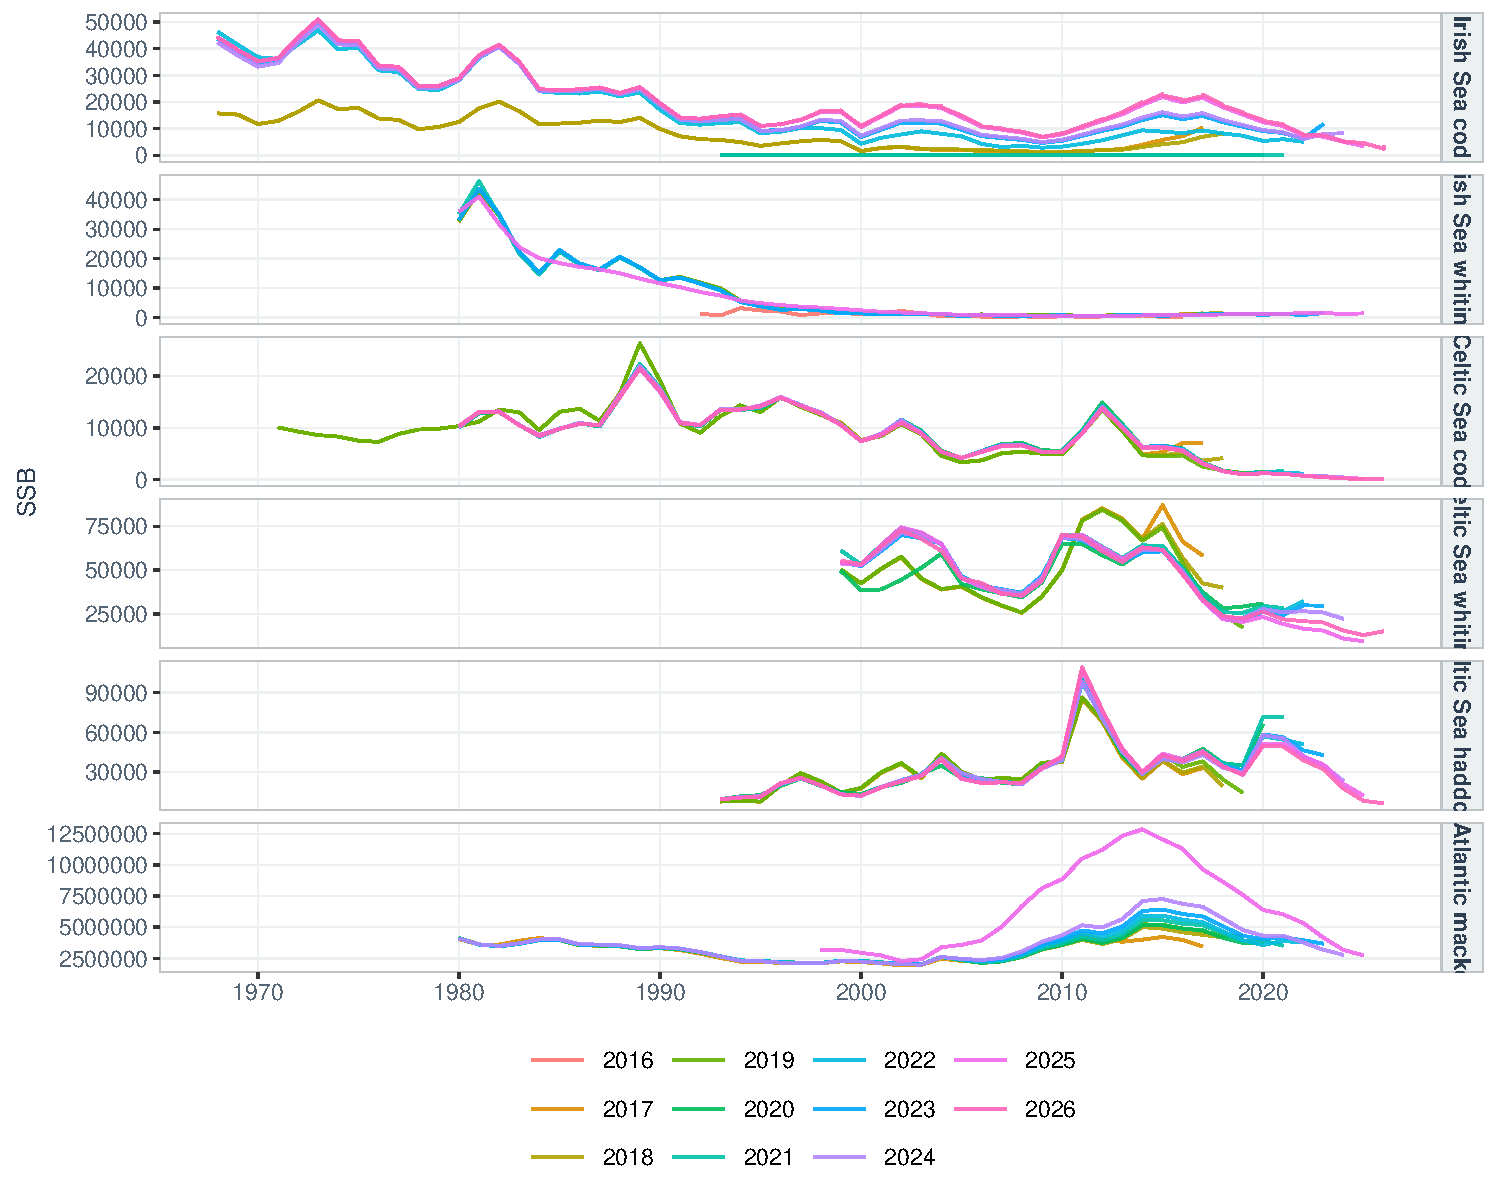
\includegraphics[width=\textwidth]{figs/week1_sag_ssb.pdf}
\caption{Spawning stock biomass by assessment year for each case-study
stock.}
\label{fig:week1-ssb}
\end{figure}

Figure~\ref{fig:week1-refpts} plots the reference points by year (\(F_{\mathrm{MSY}}\), \(B_{\lim}\),
\(B_{\mathrm{trigger}}\)) relative to the latest assessment; values near~1 indicate little revision between assessment years.


\begin{figure}[H]
\centering
\includegraphics[width=\textwidth]{figs/week1_sag_refpts.pdf}
\caption{Reference points relative to the latest assessment year
(values near 1 indicate little revision).}
\label{fig:week1-refpts}
\end{figure}

For several stocks the long-term SSB trend is similar across assessment years, with the main differences found in the terminal years --- the usual retrospective pattern that affects precision at an update. Benchmarks have
larger effects for mackerel, Celtic Sea whiting, and Irish Sea cod, where reference points or scale shift materially between assessment years. For \textbf{Northeast Atlantic mackerel}, the benchmark step changed the perceived stock scale and reference-point basis substantially. Differences between the relative trajectories may be caused by changes in the reference points, which is relatively easy to handle in the MSE by changing reference points accordingly, however for mackerel it looks like big changes have been seen also in the stock trend. Screening for mackerel should therefore be treated as provisional, and benchmark handling will be revisited in the conditioning and backtest steps

\subsection{Advice}
\label{sec:week1-advice}

Reported catch (SAG) is compared with ICES advised catch in Figure~\ref{fig:week1-catch-advice}. Years in which reported catch exceeds advice indicate periods when management did not fully implement the recommended catch. This screening comparison uses \textbf{catch versus advised catch} only; agreed TAC is not included here. TAC may be added later if needed for the full backtest; perfect-management counterfactuals already assume catch equal to advised catch with no TAC overshoot.

\begin{figure}[H]
\centering
\includegraphics[width=\textwidth]{figs/week1_catch_advice.pdf}
\caption{Reported catch (SAG) versus ICES advised catch (ASD) by calendar year
of application. Facets use independent \(y\)-axes (tonnes).}
\label{fig:week1-catch-advice}
\end{figure}

For Celtic and Irish Sea cod and whiting, advice has called for large catch reductions that were not implemented. Mackerel catches have consistently exceeded advice. Celtic Sea haddock catches have generally been below the
advised level.

\subsection{Historical projections}
\label{sec:week1-proj}

Projections (open-loop) were run over the historical period at constant target \(F = F_{\mathrm{MSY}}\) (Figure~\ref{fig:week1-proj}); these are used only for screening, not for interpretation. The panels show fishing mortality, biomass, recruitment, then catch. Three trajectories are shown for each stock; series are scaled by reference points or mean recruitment (horizontal line at~1). Catch is scaled by a simple MSY proxy,
\(MSYB_{\mathrm{trigger}}\times\bigl(1-\exp(-F_{\mathrm{MSY}})\bigr)\).
\begin{itemize}
  \item \textbf{Actual} (solid): realised \(F\) and recruitment from the
        assessment.
  \item \textbf{Target F, mean recruitment} (dashed): constant
        \(F_{\mathrm{MSY}}\) with recruitment fixed at the geometric mean
        (deterministic; no year-class deviates).
  \item \textbf{Target F, recruitment deviates} (long dash): the same constant
        \(F_{\mathrm{MSY}}\) projection with deviates from the fitted
        stock--recruitment relationship, so projected year classes follow the
        assessment.
\end{itemize}

\begin{figure}[H]
\centering
\includegraphics[width=\textwidth]{figs/week1_projections.pdf}
\caption{Actual vs.\ constant-target-\(F\) projections, scaled by SAG reference
points. Three trajectories: Actual (solid); target~\(F\),
mean recruitment (dashed; \(F_{\mathrm{MSY}}\) with geometric-mean~\(R\));
target~\(F\), recruitment deviates (long dash; same
\(F_{\mathrm{MSY}}\) with assessment deviates from the stock--recruitment
relationship). Compare dashed vs.\ long dash to isolate recruitment; compare
long dash vs.\ Actual to isolate realised~\(F\). Rows share a common
\(y\)-axis within each metric (\(F/F_{\mathrm{MSY}}\): 0--6;
SSB/\(B_{\mathrm{trigger}}\): 0--6; \(R\)/mean: 0--3; \(C\)/MSY: 0--10).
Reference lines: \(F_{\mathrm{target}}\) (green), \(B_{\mathrm{trigger}}\)
(amber, SSB row at~1), \(B_{\lim}\) (red).}
\label{fig:week1-proj}
\end{figure}


\paragraph{Separating fishing mortality and recruitment.}
The dashed and long-dash projections share the same target~\(F\), and so
isolate the effect of recruitment: any divergence in SSB, \(R\), or catch
between mean recruitment and recruitment deviates is
attributable to year-class strength, not to \(F\). Comparing
recruitment deviates to Actual uses the same recruitment
pattern but different~\(F\); divergence therefore reflects exploitation
departing from \(F_{\mathrm{MSY}}\). Comparing mean recruitment to
Actual combines both effects. This three-way contrast is for
screening only (the mean-recruitment run does not use a formal
stock--recruitment relationship); the backtest will condition operating models
on the fitted relationship and propagate deviates in projections.


\paragraph{\(F/F_{\mathrm{MSY}}\) --- exploitation level}
The top row asks whether realised~\(F\) has exceeded the MSY target. Where the
\textbf{actual} trajectory lies above~1, exploitation has exceeded
\(F_{\mathrm{MSY}}\). Celtic Sea cod, haddock, and whiting show extended
periods with \(F > F_{\mathrm{MSY}}\). Irish Sea cod has generally remained
below \(F_{\mathrm{MSY}}\); mackerel was historically below the target but is
now above \(F_{\mathrm{MSY}}\) in the latest assessment year.

\paragraph{SSB/\(B_{\mathrm{trigger}}\) --- biomass response}
The second row links fishing pressure to stock size. Stocks with sustained
\(F > F_{\mathrm{MSY}}\) tend to remain below \(B_{\mathrm{trigger}}\) or
\(B_{\lim}\), or to show substantial declines. Irish Sea whiting has increased
recently despite rising~\(F\), suggesting that recruitment or environmental
drivers may also be influencing the trajectory.

\paragraph{\(R\)/mean --- recruitment}
The dashed line (mean recruitment) is flat by construction, whereas the long-dash line varies with assessment deviates. Where mean recruitment and recruitment deviates diverge strongly, year-class strength --- rather than \(F\) alone --- drives much of the dynamics. Where the long-dash trajectory is closer to \textbf{Actual} than the dashed track, recruitment deviates help explain the historical path; where Actual differs from the long-dash run,
realised~\(F\) is the main driver.

\paragraph{\(C\)/MSY --- consequences for catch}
The bottom row translates status and recruitment into yield relative to an MSY proxy. Overfishing, poor recruitment, or both may depress realised catch.

\paragraph{Summary}
\begin{itemize}
  \item \textbf{Celtic Sea cod} --- \(F \gg F_{\mathrm{MSY}}\), SSB well below
        \(B_{\lim}\), weak recruitment; catch depressed.
  \item \textbf{Celtic Sea whiting} --- below \(B_{\mathrm{trigger}}\) with
        \(F < F_{\mathrm{MSY}}\); mean-recruitment and recruitment-deviate
        runs diverge strongly.
  \item \textbf{Celtic Sea haddock} and \textbf{mackerel} --- below
        \(B_{\mathrm{trigger}}\) with \(F > F_{\mathrm{MSY}}\) (mackerel:
        interpret with benchmark caveat above).
  \item \textbf{Irish Sea cod} --- low recent~\(F\) but biomass still poor;
        terminal SSB driven down by weak year classes since ~2020.
  \item \textbf{Irish Sea whiting} --- sparse recent SAG coverage; retained for
        the backtest with diagnostics flagged in the reconstruction step.
\end{itemize}

\paragraph{Is continuing with these six stocks worthwhile} i.e. is there a clear advice--implementation gap (Figure~\ref{fig:week1-catch-advice}), and is there evidence that following advice could improve status and yield?
The constant-\(F_{\mathrm{MSY}}\) projections provide an initial quantitative check. The next stage is to run the closed-loop backtest (contemporaneous peels and perfect-management HCR counterfactuals):
\begin{itemize}
  \item Where realised \(F\) has exceeded \(F_{\mathrm{MSY}}\) and reported
        catch has exceeded advice, constant-\(F_{\mathrm{MSY}}\) paths
        typically suggest higher SSB and, over medium horizons, more stable or
        higher cumulative yield than the depleted history---Celtic Sea cod is
        the clearest screening example.
  \item Where recent advice has been for very low or zero catch, the
        counterfactual is deliberately conservative on yield in the short
        term; the screening case for retention is then poor status and a large
        advice--catch gap, not short-term catch gains.
  \item Stocks with mixed status (below \(B_{\mathrm{trigger}}\) but
        \(F < F_{\mathrm{MSY}}\), or recovering biomass) remain useful
        contrasts for the cross-stock synthesis.
\end{itemize}

The contrasts support keeping all six stocks for a cross-stock synthesis of
non-adherence to advice. \textbf{Northeast Atlantic mackerel} is retained only
provisionally: the recent benchmark break means its status ratios, catch--advice
comparison, and projections must be revisited before conditioning. Screening projections used a geometric-mean
recruitment proxy rather than a formal stock--recruitment relationship. For the
backtest, operating models will be conditioned on assessment-consistent
stock--recruitment relationships, with recruitment deviates used to represent
year-class strength in counterfactual projections. \textbf{Proceed with all six
initial stocks}; no alternative list is proposed at this stage.

\section{Discussion}
\label{sec:week1-discussion}

The screening results illustrate four features that the backtest should separate when attributing outcomes to advice adherence versus assessment and reference-point revision.

\paragraph{Perception changes at each update or benchmark.}
SAG SSB fans (Figure~\ref{fig:week1-ssb}) show that the historical perception
of stock status is revised whenever the assessment is updated, and more
substantially at benchmarks. The same calendar year can therefore be judged
as above or below \(B_{\mathrm{trigger}}\) (or \(B_{\lim}\)) depending on
which assessment year is used. A perfect-management counterfactual that
applies advice based on the contemporaneous perception must therefore be
anchored to the assessment available \emph{at the time}, not to the latest
revised history. Comparing realised catches with advice derived from today's
assessment could conflate implementation failure with retrospective revision
of status.

\paragraph{Recruitment and the stock--recruitment relationship.}
Historical projections at fixed target~\(F\) (Figure~\ref{fig:week1-proj})
show that deterministic mean recruitment often fails to track assessed SSB and
catch, whereas runs that retain recruitment deviates from the
stock--recruitment relationship stay closer to the assessment on
recruitment-driven quantities. For several stocks, year-class strength
dominates short-term trajectories relative to the choice of target~\(F\) alone.
Conditioning the operating model will therefore centre on the
stock--recruitment relationship: its functional form, estimated parameters, and
the recruitment deviates applied in projection. The backtest should report
sensitivity to these assumptions so that differences between realised and
counterfactual paths are not attributed solely to whether advice was followed.

\paragraph{Mackerel and benchmark breaks.}
Northeast Atlantic mackerel stands out among the case studies because the
reference-point and scale revision at the recent benchmark is large relative to
other stocks. Status ratios, catch--advice comparisons, and screening
projections for mackerel should be interpreted cautiously until benchmark-year
handling (reference points, perception, and advice rule) is agreed for the
backtest peel sequence. This stock will be revisited early in the conditioning
phase.

\paragraph{Reference points change at benchmarks.}
Relative reference-point series (Figure~\ref{fig:week1-refpts}) confirm that
\(F_{\mathrm{MSY}}\), \(B_{\lim}\), and \(MSYB_{\mathrm{trigger}}\) are not
fixed for the duration of a management history: they jump when benchmarks
redefine biology, selectivity, or the basis for MSY. Advice rules coded with
today's reference points could misrepresent the harvest control rule in force
in earlier years. The backtest should carry forward the reference points
published with each assessment year (or the values used in that year's
advice) when applying the MSY rule, and treat benchmark years as structural
breaks when interpreting changes in advised \(F\) or catch.


\section{Next steps}

The following steps follow on from the screening. Reconstruct annual perceptions and advice rules as they were, project under perfect implementation, and compare with realised history. This separates assessment revision, recruitment stochasticity, and reference-point change from questions of advice adherence. Operating-model conditioning will prioritise the stock--recruitment relationship and recruitment deviates for each stock
(Section~\ref{sec:week1-discussion}).

\begin{table}[H]
\centering
\caption{Tass to conduct backtest.}
\label{tab:week1-implications}
\begin{tabular}{@{}lp{10.5cm}@{}}
\toprule
Topic & Conclusion \\
\midrule
Case studies & Keep all six proposal stocks; mackerel provisional pending benchmark handling \\
Advice rules & ICES MSY approach for gadoids; Coastal States / ICES MSY rule for mackerel \\
Catch vs advice & Screening uses catch vs advised catch; TAC not considered in Figure~\ref{fig:week1-catch-advice} \\
Backtest window & Align peels with each stock's SAG coverage, i.e. go back to 2016 \\
Stock--recruitment relationship & Key conditioning step: fit assessment-consistent relationship; use recruitment deviates in projections \\
Advice Rule & Short-term reference projections for contemporaneous assessment using reference points available at the time \\
\bottomrule
\end{tabular}
\end{table}


\begin{enumerate}
  \item \textbf{Agree the backtest peel window per stock.}
        Set start and end years based on Table~\ref{tab:week1-sagcov}. SAG
        online coverage is the binding constraint: assessment histories span
        only about 7--10 years (roughly 2016--2026) for most stocks, even
        though the local \texttt{FLStock} series run back to the 1960s--1980s.
        The effective backtest window is therefore about ten assessment years,
        which is adequate for the aims of this study and bounds how much can be
        concluded from the retrospective.
  \item \textbf{Treat benchmarks as structural breaks.}
        Flag benchmark years for reference-point and model-setting changes;
        prioritise mackerel (Section~\ref{sec:week1-discussion}).
  \item \textbf{Code contemporaneous advice rules.}
		Implement the ICES Category~1 MSY rule for gadoids and the Coastal
		States / ICES MSY rule for mackerel, using each year's published
		\(F_{\mathrm{MSY}}\), \(MSYB_{\mathrm{trigger}}\), and \(B_{\lim}\)
		(Section~\ref{sec:week1-discussion}), not a single latest set of
		reference points.
  \item \textbf{Assessment reconstruction.}
        Approximate annual perceptions by re-running SAM off the available
        inputs (most recent assessment and 2020), simulating survey CPUE where
        contemporaneous indices are missing. Because this is a simulation study
        rather than a fresh statutory assessment, the held catch-at-age and
        biological data are sufficient; genuine year-by-year re-runs are not
        required (see \emph{Feasibility and data availability} below).

  \item \textbf{Condition operating models.}
        Fit the stock--recruitment relationship for each stock (dynamic-\(B_0\)
        or assessment-equivalent form), validate recruitment deviates, and
        document sensitivity scenarios.
  \item \textbf{Perfect-management counterfactuals.}
        From each peel, apply that year's advice and project forward under
        catches equal to advised catch. Report SSB, \(F\), and catch paths
        against realised history, using the conditioned stock--recruitment
        relationship and appropriate recruitment deviates.

  \item \textbf{Stock-specific summaries and cross-stock synthesis.}
        Tabulate time below \(B_{\lim}\) and \(B_{\mathrm{trigger}}\),
        \(F\) relative to \(F_{\mathrm{MSY}}\), and yield/stability metrics for
        realised vs.\ counterfactual paths; synthesise where adherence would
        have mattered most versus where assessment or reference-point revision
        dominate.
\end{enumerate}

\paragraph{Feasibility}
The biggest task, assessment reconstruction, depends on creating the observation error model, i.e. simulation of the survey indices, catch-at-age, and biological data as they stood at each historical assessment. SAG provides only the estimated \emph{output} time series, not these inputs. This is a simulation exercise, not a statutory
re-assessment, so contemporaneous inputs need not be recovered exactly. Selectivity-at-age and biological data can be taken from the most recent assessment, and survey indices can be simulated and SAM re-run to produce plausible
contemporaneous perceptions. Two stock-specific issues remain: Irish Sea whiting has some missing SAG years (an
easy fix), and Northeast Atlantic mackerel has a large benchmark change (needs more thought).

\paragraph{Yimeline.}
These next steps map onto the project plan's Tasks~2--4---assessment reconstruction (20~days), counterfactual simulation (15~days), and comparative analysis and reporting (10~days)---about 45~days in total, following the
completed Task~1 screening (5~days). However, much more work was conducting during the screening that first envisaged; much of the code (SAG/\texttt{FLStock} for processing the ICES datasets, conditioning the operating model, projections, HCR backtests, and plotting is in place; remaining effort is for running the code, checking results, and drafting the report, so the plan remains on track.

\paragraph{Immediate actions.}
\begin{itemize}
  \item Confirm the stock list: all six candidates retained (mackerel provisional).
  \item Start assessment reconstruction for one prototype stock.
  \item Produce short-term reference projections from the most recent assessment
        (project-plan Task~1 remainder), distinct from the whole-period screening
        projections in Section~\ref{sec:week1-proj}.
  \item Revisit Northeast Atlantic mackerel: agree benchmark-year treatment and
        reference-point carry-forward before conditioning the operating model.
\end{itemize}

\newpage
\appendix

\newpage
\section{Appendix: SAG versus local \texttt{FLStock}}
\label{app:sag-fl}

Scaled trajectories from the latest SAG assessment year compared with the
local WGCSE \texttt{FLStock} objects (common SAG reference points:
SSB/\(B_{\mathrm{trigger}}\), \(F/F_{\mathrm{MSY}}\), recruitment relative to
mean SAG recruitment, and catch relative to a simple MSY proxy).

\begin{figure}[H]
\centering
\includegraphics[width=\textwidth]{figs/week1_sag_fl.pdf}
\caption{SAG vs.\ local \texttt{FLStock}, scaled by SAG reference points
(horizontal line at 1).}
\label{fig:week1-sagfl}
\end{figure}

\newpage
\section{Appendix: Software and reproducibility}
\label{app:software}

Analysis uses FLR (\texttt{FLCore}, \texttt{FLBRP}, \texttt{FLasher},
\texttt{ggplotFL}) and the \texttt{FLBacktest} / \texttt{backtest} tools
(\texttt{hcrICES}, projection and peel helpers). The notebooks write
\texttt{RData}; this note and later reports load those results.

\begin{table}[H]
\centering
\caption{Paths used for the screening deliverable.}
\begin{tabular}{@{}ll@{}}
\toprule
Path & Role \\
\midrule
\texttt{Rmd/01\_screening.Rmd} & Screening, SAG vs FLStock, target-\(F\) projections \(\rightarrow\) \texttt{01\_screening.RData} \\
\texttt{Rmd/02.0\_condition\_om.Rmd} & OM conditioning \(\rightarrow\) \texttt{03.0\_om.RData} \\
\texttt{Rmd/04.2\_closedLoop.Rmd} & HCR counterfactuals \(\rightarrow\) \texttt{03.2\_closedLoop.RData} \\
\texttt{scripts/build\_week1\_tex.R} & Regenerates tables/figures for this document \\
\texttt{tex/backtest\_screening.tex} & This deliverable \\
\texttt{data/reference/stocks.csv} & Stock metadata and advice years \\
\bottomrule
\end{tabular}
\end{table}

\newpage
\section{Appendix: Terminology}
\label{app:terms}

\begin{table}[H]
\centering
\caption{Terminology used in this document.}
\label{tab:week1-terms}
\begin{tabular}{@{}lp{11cm}@{}}
\toprule
Term & Meaning \\
\midrule
SSB & Spawning stock biomass \\
\(F\) & Fishing mortality (mean \(F\) across ages) \\
\(F_{\mathrm{MSY}}\) & MSY-related fishing mortality (from SAG when available) \\
\(F_{\mathrm{target}}\) & Target fishing mortality used in advice (from SAG when available) \\
\(B_{\mathrm{lim}}\) & Limit biomass reference point \\
\(B_{\mathrm{trigger}}\) (\(MSYB_{\mathrm{trigger}}\)) & Trigger biomass reference point \\
SAG & ICES Stock Assessment Graphs \\
ASD & ICES advice database \\
HCR & Harvest control rule \\
OM & Operating model used in MSE \\
Stock--recruitment relationship & How recruitment depends on SSB
  (the informal code abbreviation ``SRR'' is avoided in this text) \\
TAC & Total allowable catch (scoped out of the catch--advice comparison in
  Section~\ref{sec:week1-advice}) \\
\bottomrule
\end{tabular}
\end{table}

\end{document}
